% ============================================================================
%  COMPILE WITH XeLaTeX  (twice, so the point total resolves)
%  Overleaf: Menu -> Compiler -> XeLaTeX
%  Requires: bnhandout.sty and fonts/Kalpurush.ttf in the project
% ============================================================================
\documentclass[11pt]{article}
\usepackage{bnhandout}          % add [nosol] for a student edition

\hauthor[https://sites.google.com/view/jugantordey/home]{Jugantor Dey}
\hseries{Mathematics for the Physics Olympiad}

\begin{document}

\handouttitle{Chapter 20 : Vectors}

\noindent
এই অধ্যায়ে সবচেয়ে বেশি লাগবে ১২ নম্বর অধ্যায়ের অক্ষের ঘূর্ণন এবং
৭ নম্বর অধ্যায়ের কোসাইন সূত্র; ১১ নম্বর অধ্যায়ের ত্রিমাত্রিক
জ্যামিতিও কাজে লাগবে। ক্যালকুলাস এখানে প্রায় লাগবেই না, কিন্তু ২১ নম্বর
অধ্যায়ে ভেক্টর ও ক্যালকুলাস একসঙ্গে আসবে, তাই ১৫ ও ১৭ নম্বর অধ্যায়
হাতের কাছে রাখা ভালো।

ভেক্টর সম্পর্কে স্কুলে যে সংজ্ঞাটা শেখানো হয় (``মান ও দিক আছে যার'') সেটি
মনে রাখার জন্য ভালো, কিন্তু সংজ্ঞা হিসেবে দুর্বল। কেন দুর্বল, তা প্রথম অনুচ্ছেদেই দেখা যাবে: এমন জিনিস আছে যার মান ও দিক দুটোই আছে অথচ সে ভেক্টর নয়।
সঠিক সংজ্ঞাটা একটু আলাদা এবং অনেক বেশি কাজের: ভেক্টর হলো এমন বস্তু যার
উপাংশগুলো অক্ষ ঘোরালে একটি নির্দিষ্ট নিয়মে বদলায়। উপাংশ নির্ভর করে
আমরা কোন অক্ষ বেছেছি তার উপর; ভেক্টরটি নিজে করে না।

এই দৃষ্টিভঙ্গিটা পদার্থবিজ্ঞানে কেন এত গুরুত্বপূর্ণ, তার কারণ সহজ। ভৌত নিয়ম
কোনো নির্দিষ্ট স্থানাঙ্ক ব্যবস্থার উপর নির্ভর করতে পারে না; কে কোন দিকে অক্ষ
বসাল তাতে প্রকৃতির কিছু যায় আসে না। তাই নিয়মগুলো ভেক্টর সমীকরণে লিখলে সেগুলো
আপনা থেকেই সব ব্যবস্থায় একই থাকে।

এই অধ্যায়ে মোট \totalpoints\ পয়েন্ট আছে।

\section{ভেক্টর কী}

কিছু ভৌত রাশি বর্ণনা করতে একটিমাত্র সংখ্যা যথেষ্ট: ভর, তাপমাত্রা, সময়, আধান।
এদের বলে scalar। আবার কিছু রাশির জন্য সংখ্যার পাশাপাশি দিকও লাগে: সরণ, বেগ,
বল, বৈদ্যুতিক ক্ষেত্র। এদের বলে vector।

কিন্তু ``মান ও দিক'' পরীক্ষাটা যথেষ্ট নয়।

\begin{remark}
একটি বই টেবিলে রাখো। এবার তাকে $x$-অক্ষ ঘিরে $90^{\circ}$ ঘোরাও, তারপর
$y$-অক্ষ ঘিরে $90^{\circ}$ ঘোরাও; বইটি যে অবস্থায় দাঁড়াল তা মনে রাখো। এখন
আবার শুরু থেকে করো, কিন্তু এবার আগে $y$ ঘিরে, তারপর $x$ ঘিরে। দুটি চূড়ান্ত
অবস্থা এক নয়।

অথচ প্রতিটি ঘূর্ণনের একটি মান আছে (কোণ) এবং একটি দিক আছে (অক্ষ)। যদি ঘূর্ণন
ভেক্টর হতো, তবে তাদের যোগ করা যেত এবং ক্রম বদলালেও ফল একই হতো, কারণ ভেক্টর
যোগ বিনিময়যোগ্য। তা হচ্ছে না, তাই সসীম ঘূর্ণন ভেক্টর নয়।

(খুব ছোট ঘূর্ণনের ক্ষেত্রে ব্যাপারটা আলাদা; তখন ক্রম বদলালে যে পার্থক্য হয় তা
উচ্চতর ক্রমের, আর সেই কারণেই কৌণিক বেগ ভেক্টর।)
\end{remark}

তাহলে সঠিক সংজ্ঞা কী?

\begin{idea}[ভেক্টরের সংজ্ঞা]
তিনটি সংখ্যার একটি সেট $\left( A_{x}, A_{y}, A_{z} \right)$ ভেক্টরের উপাংশ
বলে গণ্য হবে যদি অক্ষ ঘোরালে তারা ঠিক সেই নিয়মে বদলায় যে নিয়মে অবস্থান
স্থানাঙ্ক বদলায়।

দুই মাত্রায়, ১২ নম্বর অধ্যায় অনুযায়ী অক্ষ $\theta$ কোণে ঘোরালে
\[
  A_{x}' = A_{x}\cos\theta + A_{y}\sin\theta, \qquad
  A_{y}' = -A_{x}\sin\theta + A_{y}\cos\theta .
\]
\end{idea}

লক্ষ করো এখানে কী দাবি করা হচ্ছে। ভেক্টরটি নড়েনি; কেবল আমরা অন্য চোখে দেখছি,
তাই তার উপাংশগুলোর নাম বদলেছে। যা বদলায়নি তা হলো ভেক্টরটি নিজে, এবং তার
দৈর্ঘ্য (এই অনুচ্ছেদের শেষ সমস্যাটি দেখো)।

সংকেত: ভেক্টর লেখা হয় মোটা অক্ষরে $\mathbf{A}$ অথবা তীরচিহ্ন দিয়ে
$\vec{A}$; তার মান $|\mathbf{A}|$ বা সংক্ষেপে $A$। দুটি ভেক্টর সমান তখনই,
যখন তাদের সব উপাংশ সমান।

\begin{example}
দুই মাত্রায় $\mathbf{A} = (1,0)$ নাও এবং অক্ষ $45^{\circ}$ ঘোরাও। নতুন উপাংশ
বের করো, এবং দেখাও যে দৈর্ঘ্য বদলায়নি।
\end{example}

\begin{solbox}
$\cos 45^{\circ} = \sin 45^{\circ} = \dfrac{1}{\sqrt{2}}$ বসিয়ে
\[
  A_{x}' = 1 \cdot \frac{1}{\sqrt{2}} + 0 = \frac{1}{\sqrt{2}}, \qquad
  A_{y}' = -1 \cdot \frac{1}{\sqrt{2}} + 0 = -\frac{1}{\sqrt{2}} .
\]
দৈর্ঘ্য:
\[
  \sqrt{A_{x}'^{2} + A_{y}'^{2}} = \sqrt{\tfrac{1}{2}+\tfrac{1}{2}} = 1
  = \sqrt{A_{x}^{2}+A_{y}^{2}} .
\]
১২ নম্বর অধ্যায়ে সাধারণভাবে প্রমাণ করা হয়েছিল যে ঘূর্ণনে $x^{2}+y^{2}$
বদলায় না; এখানে সেটিই আবার কাজে লাগল।
\end{solbox}

\prob{2} নিচের কোনগুলো ভেক্টর ও কোনগুলো scalar: তাপমাত্রা, বেগ, দ্রুতি,
সরণ, ভর, বৈদ্যুতিক ক্ষেত্র, চাপ, তড়িৎপ্রবাহ? শেষটির ক্ষেত্রে সাবধানতাটি
আলাদা করে ব্যাখ্যা করো।

\begin{sol}
Vector: বেগ, সরণ, বৈদ্যুতিক ক্ষেত্র।

Scalar: তাপমাত্রা, দ্রুতি, ভর, চাপ, তড়িৎপ্রবাহ।

তড়িৎপ্রবাহ নিয়ে সাবধানতা: তারের মধ্যে প্রবাহের একটি ``দিক'' আছে বলে অনেকে
একে ভেক্টর ভাবে। কিন্তু প্রবাহ যোগ হয় সাধারণ সংখ্যার মতো (Kirchhoff-এর
সংযোগ-বিধি), ভেক্টরের মতো নয়; দুটি তার এক জায়গায় মিললে প্রবাহ দুটি
সামান্তরিক নিয়মে যোগ হয় না। তাই তড়িৎপ্রবাহ scalar। যেটি সত্যিকারের ভেক্টর
সেটি হলো প্রবাহ ঘনত্ব।

দ্রুতি ও বেগের পার্থক্যও একই ধরনের: দ্রুতি হলো বেগের মান, তাই scalar।
\end{sol}

\prob{3} দুই মাত্রায় অক্ষ $45^{\circ}$ ঘোরানো হলো এবং বিন্দুটি $(1,0)$।
\begin{enumerate}
  \item $(x,y)$ জোড়াটি ভেক্টরের নিয়ম মানে কি না দেখাও।
  \item $\left( x^{2}, y^{2} \right)$ জোড়াটি একই নিয়ম মানে কি না পরীক্ষা
        করো, এবং ফল থেকে কী সিদ্ধান্ত হয় বলো।
\end{enumerate}

\begin{sol}
\begin{enumerate}
  \item সংজ্ঞা অনুযায়ীই $(x,y)$ ওই নিয়মে বদলায়; উপরের উদাহরণে
        $(x', y') = \left( \tfrac{1}{\sqrt{2}}, -\tfrac{1}{\sqrt{2}} \right)$।
  \item মূল জোড়াটি $\left( x^{2}, y^{2} \right) = (1, 0)$। ভেক্টরের নিয়ম
        খাটলে নতুন জোড়া হতো
        $\left( \tfrac{1}{\sqrt{2}}, -\tfrac{1}{\sqrt{2}} \right)
        \approx (0.707, -0.707)$।

        কিন্তু প্রকৃত মান হলো $\left( (x')^{2}, (y')^{2} \right)
        = \left( \tfrac{1}{2}, \tfrac{1}{2} \right)$।

        দুটি মেলে না, তাই $\left( x^{2}, y^{2} \right)$ ভেক্টর নয়।
\end{enumerate}
সিদ্ধান্ত: দুটি সংখ্যা পাশাপাশি লিখে বন্ধনীতে রাখলেই তা ভেক্টর হয়ে যায় না।
রূপান্তরের নিয়মটাই আসল পরীক্ষা।
\end{sol}

\section{উপাংশ ও অভিক্ষেপ}

\begin{idea}[একক ভেক্টর ও উপাংশ]
$\hat{\mathbf{x}}, \hat{\mathbf{y}}, \hat{\mathbf{z}}$ দিয়ে বোঝানো হয় তিনটি
অক্ষ বরাবর একক দৈর্ঘ্যের ভেক্টর। তখন যেকোনো ভেক্টর
\[
  \mathbf{A} = A_{x}\hat{\mathbf{x}} + A_{y}\hat{\mathbf{y}}
             + A_{z}\hat{\mathbf{z}} ,
\]
এবং ১১ নম্বর অধ্যায়ের ত্রিমাত্রিক Pythagoras অনুযায়ী
\[
  |\mathbf{A}| = \sqrt{A_{x}^{2}+A_{y}^{2}+A_{z}^{2}} .
\]
$\mathbf{A}$-এর দিকের একক ভেক্টর
$\hat{\mathbf{A}} = \dfrac{\mathbf{A}}{|\mathbf{A}|}$।
\end{idea}

কিছু বইয়ে $\hat{\mathbf{x}}, \hat{\mathbf{y}}, \hat{\mathbf{z}}$-এর বদলে
$\mathbf{i}, \mathbf{j}, \mathbf{k}$ লেখা হয়; একই জিনিস। এই সিরিজে প্রথম
রূপটি ব্যবহার করা হবে, কারণ ২১ নম্বর অধ্যায়ে অন্য স্থানাঙ্কেও একক ভেক্টর
লাগবে এবং তখন $\hat{\mathbf{r}}$, $\hat{\boldsymbol{\theta}}$ ধরনের নাম
স্বাভাবিক হয়।

\begin{center}
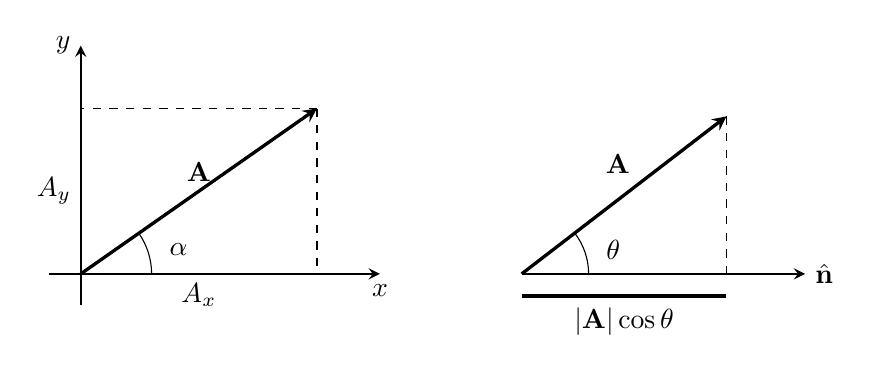
\begin{tikzpicture}[x=1.0cm,y=1.0cm,>=stealth]
 \begin{scope}
  \draw[thick,->] (-0.4,0) -- (3.8,0) node[below] {$x$};
  \draw[thick,->] (0,-0.4) -- (0,2.9) node[left] {$y$};
  \draw[very thick,->] (0,0) -- (3,2.1);
  \draw[dashed] (3,2.1) -- (3,0); \draw[dashed] (3,2.1) -- (0,2.1);
  \node[above] at (1.5,1.05) {$\mathbf{A}$};
  \node[below] at (1.5,0) {$A_{x}$};
  \node[left] at (0,1.05) {$A_{y}$};
  \draw[thin] (0.9,0) arc[start angle=0,end angle=35,radius=0.9];
  \node[right] at (17:1.05) {$\alpha$};
 \end{scope}
 \begin{scope}[xshift=5.6cm]
  \draw[very thick,->] (0,0) -- (2.6,2.0);
  \draw[thick,->] (0,0) -- (3.6,0) node[right] {$\hat{\mathbf{n}}$};
  \draw[dashed] (2.6,2.0) -- (2.6,0);
  \draw[very thick] (0,-0.28) -- (2.6,-0.28);
  \node[below] at (1.3,-0.3) {$|\mathbf{A}|\cos\theta$};
  \node[above left] at (1.5,1.15) {$\mathbf{A}$};
  \draw[thin] (0.85,0) arc[start angle=0,end angle=37.6,radius=0.85];
  \node[right] at (18:1.0) {$\theta$};
 \end{scope}
\end{tikzpicture}
\end{center}

\begin{idea}[অভিক্ষেপ]
$\hat{\mathbf{n}}$ দিকে $\mathbf{A}$-এর অভিক্ষেপ (projection) হলো
\[
  A_{n} = |\mathbf{A}|\cos\theta ,
\]
যেখানে $\theta$ হলো $\mathbf{A}$ ও $\hat{\mathbf{n}}$-এর মধ্যেকার কোণ।
উপাংশ আসলে অভিক্ষেপেরই বিশেষ ক্ষেত্র: $A_{x}$ হলো $\hat{\mathbf{x}}$ দিকে
অভিক্ষেপ।
\end{idea}

ছবির ডান পাশে ব্যাপারটা দেখা যাচ্ছে: $\mathbf{A}$-এর মাথা থেকে
$\hat{\mathbf{n}}$-এর উপর লম্ব ফেললে যে দৈর্ঘ্য কাটা পড়ে, সেটিই অভিক্ষেপ।
$\theta$ স্থূলকোণ হলে $\cos\theta$ ঋণাত্মক, অর্থাৎ অভিক্ষেপও ঋণাত্মক; সেটি
ঠিকই আছে, কারণ তখন $\mathbf{A}$ উল্টো দিকে হেলে আছে।

\begin{example}
$\mathbf{A} = 6\hat{\mathbf{x}} - 3\hat{\mathbf{y}} + 2\hat{\mathbf{z}}$
হলে $|\mathbf{A}|$, $\hat{\mathbf{A}}$ এবং $x$-অক্ষের সঙ্গে $\mathbf{A}$-এর
কোণ নির্ণয় করো।
\end{example}

\begin{solbox}
\[
  |\mathbf{A}| = \sqrt{36+9+4} = \sqrt{49} = 7 .
\]
\[
  \hat{\mathbf{A}} = \frac{1}{7}\left( 6\hat{\mathbf{x}}
  - 3\hat{\mathbf{y}} + 2\hat{\mathbf{z}} \right) .
\]
$x$-অক্ষের সঙ্গে কোণ $\alpha$ হলে $A_{x} = |\mathbf{A}|\cos\alpha$, তাই
\[
  \cos\alpha = \frac{6}{7} \;\Longrightarrow\; \alpha \approx 31.0^{\circ} .
\]
এই $\cos\alpha$-কে বলে direction cosine, আর তিনটি অক্ষের জন্য তিনটি
direction cosine পাওয়া যায়।
\end{solbox}

\prob{2} \begin{enumerate}
  \item $xy$-সমতলে $20$ একক মানের একটি ভেক্টর $x$-অক্ষের সঙ্গে $60^{\circ}$
        কোণ করে। উপাংশ নির্ণয় করো।
  \item $\mathbf{B} = 3\hat{\mathbf{x}} - 4\hat{\mathbf{y}}
        + 12\hat{\mathbf{z}}$-এর মান ও একক ভেক্টর নির্ণয় করো।
\end{enumerate}

\begin{sol}
\begin{enumerate}
  \item $B_{x} = 20\cos 60^{\circ} = 10$ এবং
        $B_{y} = 20\sin 60^{\circ} = 10\sqrt{3} \approx 17.3$।
  \item $|\mathbf{B}| = \sqrt{9+16+144} = \sqrt{169} = 13$, তাই
        \[
          \hat{\mathbf{B}} = \frac{3}{13}\hat{\mathbf{x}}
          - \frac{4}{13}\hat{\mathbf{y}} + \frac{12}{13}\hat{\mathbf{z}} .
        \]
        যাচাই: $\dfrac{9+16+144}{169} = 1$।
\end{enumerate}
\end{sol}

\prob{3} $\mathbf{A}$ যদি তিন অক্ষের সঙ্গে যথাক্রমে $\alpha, \beta, \gamma$
কোণ করে, প্রমাণ করো যে
\[
  \cos^{2}\alpha + \cos^{2}\beta + \cos^{2}\gamma = 1 .
\]
এখান থেকে বলো, একটি ভেক্টর কি তিনটি অক্ষের সঙ্গেই $45^{\circ}$ কোণ করতে পারে?

\begin{sol}
সংজ্ঞা অনুযায়ী $A_{x} = |\mathbf{A}|\cos\alpha$ এবং একইভাবে বাকি দুটি। তাই
\[
  A_{x}^{2}+A_{y}^{2}+A_{z}^{2}
  = |\mathbf{A}|^{2}\left( \cos^{2}\alpha + \cos^{2}\beta
  + \cos^{2}\gamma \right) .
\]
কিন্তু বাম পাশ $|\mathbf{A}|^{2}$, তাই বন্ধনীর ভেতরের রাশিটি $1$।

$45^{\circ}$ সম্ভব নয়: তখন প্রতিটি $\cos^{2} = \tfrac{1}{2}$ হতো এবং যোগফল
$\tfrac{3}{2} \neq 1$। তিন অক্ষের সঙ্গে সমান কোণ করতে হলে
$\cos^{2} = \tfrac{1}{3}$, অর্থাৎ কোণটি প্রায় $54.7^{\circ}$; এটিই ঘনকের
কর্ণের কোণ।
\end{sol}

\newpage

\section{যোগ ও বিয়োগ}

\begin{idea}[যোগের দুই রূপ]
জ্যামিতিকভাবে: $\mathbf{B}$-এর লেজ $\mathbf{A}$-এর মাথায় বসাও; তখন
$\mathbf{A}$-এর লেজ থেকে $\mathbf{B}$-এর মাথা পর্যন্ত ভেক্টরটিই
$\mathbf{A}+\mathbf{B}$। সমতুল্যভাবে দুটিকে বাহু ধরে সামান্তরিক আঁকলে কর্ণটিই
যোগফল।

উপাংশে:
\[
  \mathbf{A}+\mathbf{B} = \left( A_{x}+B_{x} \right)\hat{\mathbf{x}}
  + \left( A_{y}+B_{y} \right)\hat{\mathbf{y}}
  + \left( A_{z}+B_{z} \right)\hat{\mathbf{z}} .
\]
যোগ বিনিময়যোগ্য ও সংযোগযোগ্য, আর $\mathbf{A}-\mathbf{B}$ মানে
$\mathbf{A}+(-\mathbf{B})$।
\end{idea}

\begin{center}
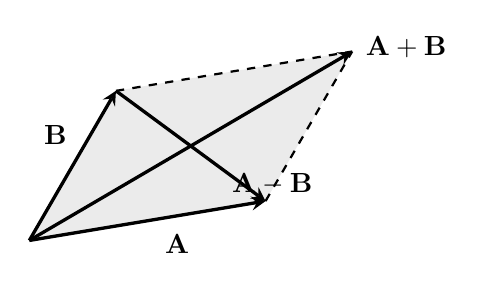
\begin{tikzpicture}[x=1.0cm,y=1.0cm,>=stealth]
  \fill[black!8] (0,0) -- (3,0.5) -- (4.1,2.4) -- (1.1,1.9) -- cycle;
  \draw[very thick,->] (0,0) -- (3,0.5); \node[below right] at (1.6,0.2) {$\mathbf{A}$};
  \draw[very thick,->] (0,0) -- (1.1,1.9); \node[above left] at (0.6,1.1) {$\mathbf{B}$};
  \draw[thick,dashed] (3,0.5) -- (4.1,2.4);
  \draw[thick,dashed] (1.1,1.9) -- (4.1,2.4);
  \draw[very thick,->] (0,0) -- (4.1,2.4);
  \node[right] at (4.15,2.45) {$\mathbf{A}+\mathbf{B}$};
  \draw[very thick,->] (1.1,1.9) -- (3,0.5);
  \node[below right] at (2.45,0.98) {$\mathbf{A}-\mathbf{B}$};
\end{tikzpicture}
\end{center}

খেয়াল করো $\mathbf{A}-\mathbf{B}$ কোথায় বসেছে: সামান্তরিকের অন্য কর্ণ,
$\mathbf{B}$-এর মাথা থেকে $\mathbf{A}$-এর মাথার দিকে। এটি মনে রাখার সহজ উপায়:
$\mathbf{B} + (\mathbf{A}-\mathbf{B}) = \mathbf{A}$, তাই তীরটি অবশ্যই
$\mathbf{B}$-এর মাথা থেকে $\mathbf{A}$-এর মাথায় যাবে।

দুটি ভেক্টরের যোগফলের মান বের করতে ৭ নম্বর অধ্যায়ের কোসাইন সূত্র লাগে।
$\mathbf{A}$ ও $\mathbf{B}$-এর মধ্যেকার কোণ $\theta$ হলে
\[
  |\mathbf{A}+\mathbf{B}|^{2}
  = A^{2} + B^{2} + 2AB\cos\theta .
\]
(ত্রিভুজে কোসাইন সূত্রে বিয়োগ থাকে, এখানে যোগ, কারণ ত্রিভুজের ভেতরের কোণটি
$180^{\circ}-\theta$।)

\begin{remark}
৯ নম্বর অধ্যায়ে ত্রিভুজ অসমতা প্রমাণ করে বলা হয়েছিল যে এটি ২০ নম্বর
অধ্যায়ে ভেক্টর আকারে ফিরে আসবে। এসেছে:
\[
  |\mathbf{A}+\mathbf{B}| \leq |\mathbf{A}| + |\mathbf{B}| .
\]
উপরের সূত্র থেকেই দেখা যায়, কারণ $\cos\theta \leq 1$, তাই
$|\mathbf{A}+\mathbf{B}|^{2} \leq A^{2}+B^{2}+2AB = (A+B)^{2}$। সমতা ঘটে
কেবল $\theta = 0$-এ, অর্থাৎ দুটি ভেক্টর একই দিকে থাকলে; ৯ নম্বর অধ্যায়ে
ঠিক এই কথাই বলা হয়েছিল।
\end{remark}

\begin{example}
$\mathbf{A} = 2\hat{\mathbf{x}}+3\hat{\mathbf{y}}-\hat{\mathbf{z}}$ ও
$\mathbf{B} = -\hat{\mathbf{x}}+\hat{\mathbf{y}}+4\hat{\mathbf{z}}$ হলে
$\mathbf{A}+\mathbf{B}$ ও $2\mathbf{A}-3\mathbf{B}$ নির্ণয় করো।
\end{example}

\begin{solbox}
উপাংশে যোগ করি:
\[
  \mathbf{A}+\mathbf{B} = \hat{\mathbf{x}} + 4\hat{\mathbf{y}}
  + 3\hat{\mathbf{z}} .
\]
আর
\[
  2\mathbf{A} = 4\hat{\mathbf{x}}+6\hat{\mathbf{y}}-2\hat{\mathbf{z}},
  \qquad
  3\mathbf{B} = -3\hat{\mathbf{x}}+3\hat{\mathbf{y}}+12\hat{\mathbf{z}} ,
\]
তাই
\[
  2\mathbf{A}-3\mathbf{B} = 7\hat{\mathbf{x}} + 3\hat{\mathbf{y}}
  - 14\hat{\mathbf{z}} .
\]
\end{solbox}

\prob{2} উপরের $\mathbf{A}$ ও $\mathbf{B}$-এর জন্য
$\mathbf{A}-\mathbf{B}$ এবং $|\mathbf{A}+\mathbf{B}|$ নির্ণয় করো।

\begin{sol}
\[
  \mathbf{A}-\mathbf{B} = 3\hat{\mathbf{x}} + 2\hat{\mathbf{y}}
  - 5\hat{\mathbf{z}} .
\]
আগের উদাহরণ থেকে $\mathbf{A}+\mathbf{B} = (1,4,3)$, তাই
\[
  |\mathbf{A}+\mathbf{B}| = \sqrt{1+16+9} = \sqrt{26} \approx 5.10 .
\]
\end{sol}

\prob{3} $5$ N ও $8$ N মানের দুটি বল একই বিন্দুতে $60^{\circ}$ কোণে কাজ
করছে। লব্ধির মান এবং $5$ N বলের সঙ্গে লব্ধির কোণ নির্ণয় করো।

\begin{sol}
মান:
\[
  R^{2} = 5^{2} + 8^{2} + 2(5)(8)\cos 60^{\circ} = 25+64+40 = 129 ,
\]
তাই $R = \sqrt{129} \approx 11.36$ N।

কোণ: $5$ N বলকে $x$-অক্ষ ধরি। তখন লব্ধির উপাংশ
\[
  R_{x} = 5 + 8\cos 60^{\circ} = 9, \qquad
  R_{y} = 8\sin 60^{\circ} = 6.93 .
\]
সুতরাং $\tan\alpha = \dfrac{6.93}{9} = 0.770$, অর্থাৎ
$\alpha \approx 37.6^{\circ}$।

যাচাই: $\sqrt{81 + 48} = \sqrt{129}$, মানের সঙ্গে মিলছে। আর কোণটি
$0$ ও $60^{\circ}$-এর মাঝে, বড় বলটির দিকে হেলে; সেটাই প্রত্যাশিত।
\end{sol}

\section{ডট গুণন}

দুটি ভেক্টর গুণ করার দুটি অর্থপূর্ণ উপায় আছে। প্রথমটির ফল একটি scalar।

\begin{idea}[Dot product]
\[
  \mathbf{A}\cdot\mathbf{B} = |\mathbf{A}||\mathbf{B}|\cos\theta
  = A_{x}B_{x} + A_{y}B_{y} + A_{z}B_{z} ,
\]
যেখানে $\theta$ ভেক্টর দুটির মধ্যেকার কোণ। এটি বিনিময়যোগ্য ও বণ্টনযোগ্য, আর
$\mathbf{A}\cdot\mathbf{A} = |\mathbf{A}|^{2}$।
\end{idea}

দুটি রূপ যে এক, তা কোসাইন সূত্র থেকে বেরোয়। $\mathbf{A}-\mathbf{B}$
ভেক্টরটির দৈর্ঘ্য দুইভাবে লিখি। একদিকে কোসাইন সূত্র (৭ নম্বর অধ্যায়):
\[
  |\mathbf{A}-\mathbf{B}|^{2} = A^{2}+B^{2}-2AB\cos\theta .
\]
অন্যদিকে উপাংশে:
\[
  |\mathbf{A}-\mathbf{B}|^{2} = \sum_{i}\left( A_{i}-B_{i} \right)^{2}
  = \sum_{i}A_{i}^{2} + \sum_{i}B_{i}^{2} - 2\sum_{i}A_{i}B_{i}
  = A^{2}+B^{2} - 2\sum_{i}A_{i}B_{i} .
\]
দুটি তুলনা করলে $AB\cos\theta = \sum_{i}A_{i}B_{i}$।

\begin{idea}[জ্যামিতিক অর্থ]
Dot product মাপে দুটি ভেক্টর কতটা \emph{একই দিকে} আছে।
অর্থাৎ $\mathbf{A}\cdot\mathbf{B}$ হলো $|\mathbf{A}|$ গুণ
$\hat{\mathbf{A}}$ দিকে $\mathbf{B}$-এর অভিক্ষেপ।
বিশেষ করে $\mathbf{A}\cdot\mathbf{B} = 0$ হয় ঠিক তখনই, যখন দুটি ভেক্টর
পরস্পর লম্ব (কোনোটি শূন্য না হলে)। আর $\hat{\mathbf{n}}$ দিকে অভিক্ষেপ
লেখা যায় সংক্ষেপে $\mathbf{A}\cdot\hat{\mathbf{n}}$।
\end{idea}

পদার্থবিজ্ঞানে যেখানেই ``কতটুকু অংশ ওই দিকে'' জাতীয় প্রশ্ন আসে, সেখানেই dot
product। কৃতকাজ $W = \mathbf{F}\cdot\mathbf{d}$: বল ও সরণ লম্ব হলে কাজ শূন্য,
যা চেনা কথা। ২১ নম্বর অধ্যায়ে flux $\mathbf{E}\cdot d\mathbf{A}$ একই
ধারণা।

\begin{remark}
৯ নম্বর অধ্যায়ের আরেকটি ধার এখানে শোধ হয়। সেখানে কোশি-শোয়ার্জ অসমতা
$\left( \sum a_{i}b_{i} \right)^{2} \leq \left( \sum a_{i}^{2} \right)
\left( \sum b_{i}^{2} \right)$ প্রমাণ করে বলা হয়েছিল যে ২০ নম্বর
অধ্যায়ে এর আসল চেহারা ধরা পড়বে। এখন স্পষ্ট: বাম পাশ
$\left( \mathbf{A}\cdot\mathbf{B} \right)^{2}$ আর ডান পাশ
$|\mathbf{A}|^{2}|\mathbf{B}|^{2}$, আর অসমতাটি নিছক $\cos^{2}\theta \leq 1$।
সমতার শর্ত (দুই সারি সমানুপাতিক) মানে দুটি ভেক্টর সমান্তরাল। যে বীজগাণিতিক
কসরত সেখানে করতে হয়েছিল, তা আসলে একটি কোণের কথাই বলছিল।
\end{remark}

\begin{example}
$\mathbf{A} = \hat{\mathbf{x}}+2\hat{\mathbf{y}}+2\hat{\mathbf{z}}$ ও
$\mathbf{B} = 2\hat{\mathbf{x}}-\hat{\mathbf{y}}+2\hat{\mathbf{z}}$-এর
মধ্যেকার কোণ, এবং $\mathbf{B}$ বরাবর $\mathbf{A}$-এর অভিক্ষেপ নির্ণয় করো।
\end{example}

\begin{solbox}
\[
  \mathbf{A}\cdot\mathbf{B} = 2 - 2 + 4 = 4 .
\]
$|\mathbf{A}| = \sqrt{1+4+4} = 3$ এবং $|\mathbf{B}| = \sqrt{4+1+4} = 3$, তাই
\[
  \cos\theta = \frac{4}{9} \;\Longrightarrow\; \theta \approx 63.6^{\circ} .
\]
অভিক্ষেপ:
\[
  \mathbf{A}\cdot\hat{\mathbf{B}} = \frac{\mathbf{A}\cdot\mathbf{B}}
  {|\mathbf{B}|} = \frac{4}{3} .
\]
\end{solbox}

\prob{2} $\mathbf{A} = 4\hat{\mathbf{x}}-\hat{\mathbf{y}}+3\hat{\mathbf{z}}$
ও $\mathbf{B} = \hat{\mathbf{x}}+2\hat{\mathbf{y}}-2\hat{\mathbf{z}}$-এর
জন্য $\mathbf{A}\cdot\mathbf{B}$, তাদের মধ্যেকার কোণ, এবং $\mathbf{B}$ বরাবর
$\mathbf{A}$-এর অভিক্ষেপ নির্ণয় করো।

\begin{sol}
\[
  \mathbf{A}\cdot\mathbf{B} = 4 - 2 - 6 = -4 .
\]
$|\mathbf{A}| = \sqrt{16+1+9} = \sqrt{26} \approx 5.099$ এবং
$|\mathbf{B}| = \sqrt{1+4+4} = 3$। সুতরাং
\[
  \cos\theta = \frac{-4}{3\sqrt{26}} \approx -0.2615
  \;\Longrightarrow\; \theta \approx 105.2^{\circ} .
\]
অভিক্ষেপ $= \dfrac{-4}{3} \approx -1.33$।

ঋণাত্মক চিহ্নটি অর্থপূর্ণ: কোণ স্থূল, তাই $\mathbf{A}$-এর অংশটি
$\mathbf{B}$-এর উল্টো দিকে।
\end{sol}

\prob{3} \begin{enumerate}
  \item প্রমাণ করো যে $\mathbf{A}\cdot\mathbf{B} = 0$ হওয়া এবং দুটি ভেক্টর
        লম্ব হওয়া একই কথা (কোনোটি শূন্য না হলে)।
  \item $\lambda$-এর কোন মানের জন্য $(2, \lambda, 1)$ ও $(3,-1,2)$ পরস্পর
        লম্ব?
\end{enumerate}

\begin{sol}
\begin{enumerate}
  \item $\mathbf{A}\cdot\mathbf{B} = |\mathbf{A}||\mathbf{B}|\cos\theta$।
        দুটি মান অশূন্য, তাই গুণফল শূন্য হওয়া আর $\cos\theta = 0$ হওয়া একই
        কথা, অর্থাৎ $\theta = 90^{\circ}$।
  \item $6 - \lambda + 2 = 0$ দেয় $\lambda = 8$।
\end{enumerate}
\end{sol}

\prob{3} কোসাইন সূত্র ব্যবহার করে প্রমাণ করো যে
$|\mathbf{A}||\mathbf{B}|\cos\theta = A_{x}B_{x}+A_{y}B_{y}+A_{z}B_{z}$।
এরপর এখান থেকে কোশি-শোয়ার্জ অসমতা বের করো এবং সমতার শর্ত বলো।

\begin{sol}
প্রমাণটি উপরে দেওয়া হয়েছে: $|\mathbf{A}-\mathbf{B}|^{2}$ রাশিটিকে একবার
কোসাইন সূত্রে ও একবার উপাংশে লিখে তুলনা করলেই ফল আসে।

কোশি-শোয়ার্জ: $|\cos\theta| \leq 1$, তাই
\[
  \left| \mathbf{A}\cdot\mathbf{B} \right|
  = |\mathbf{A}||\mathbf{B}|\left| \cos\theta \right|
  \leq |\mathbf{A}||\mathbf{B}| .
\]
উপাংশে লিখলে এটিই
$\left| \sum A_{i}B_{i} \right| \leq \sqrt{\sum A_{i}^{2}}
\sqrt{\sum B_{i}^{2}}$, অর্থাৎ ৯ নম্বর অধ্যায়ের অসমতা।

সমতা ঘটে যখন $|\cos\theta| = 1$, অর্থাৎ $\theta = 0$ বা $180^{\circ}$,
অর্থাৎ দুটি ভেক্টর সমান্তরাল। ৯ নম্বর অধ্যায়ে শর্তটি লেখা হয়েছিল
``দুই সারি সমানুপাতিক''; একই কথা।
\end{sol}

\section{ক্রস গুণন}

দ্বিতীয় ধরনের গুণনের ফল একটি ভেক্টর, এবং সেটি কেবল তিন মাত্রাতেই সংজ্ঞায়িত।

\begin{idea}[Cross product]
\[
  \left| \mathbf{A}\times\mathbf{B} \right|
  = |\mathbf{A}||\mathbf{B}|\sin\theta ,
\]
আর দিক হলো $\mathbf{A}$ ও $\mathbf{B}$ যে সমতল নির্ধারণ করে তার উপর লম্ব,
ডান হাতের নিয়ম অনুযায়ী: ডান হাতের আঙুলগুলো $\mathbf{A}$ থেকে $\mathbf{B}$-এর
দিকে ঘোরালে বুড়ো আঙুল যেদিকে থাকে।
\end{idea}

\begin{center}
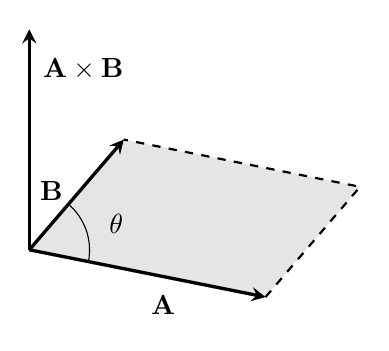
\begin{tikzpicture}[x=1.0cm,y=1.0cm,>=stealth]
  \fill[black!10] (0,0) -- (3,-0.6) -- (4.2,0.8) -- (1.2,1.4) -- cycle;
  \draw[very thick,->] (0,0) -- (3,-0.6); \node[below] at (1.7,-0.45) {$\mathbf{A}$};
  \draw[very thick,->] (0,0) -- (1.2,1.4); \node[left] at (0.55,0.75) {$\mathbf{B}$};
  \draw[thick,dashed] (3,-0.6) -- (4.2,0.8) -- (1.2,1.4);
  \draw[very thick,->] (0,0) -- (0,2.8);
  \node[right] at (0.05,2.3) {$\mathbf{A}\times\mathbf{B}$};
  \draw[thin] (0.75,-0.15) arc[start angle=-11.3,end angle=49.4,radius=0.76];
  \node[right] at (20:0.95) {$\theta$};
\end{tikzpicture}
\end{center}

জ্যামিতিক অর্থ ছবিতেই আছে: $|\mathbf{A}||\mathbf{B}|\sin\theta$ হলো
$\mathbf{A}$ ও $\mathbf{B}$ বাহুবিশিষ্ট সামান্তরিকের ক্ষেত্রফল (ভূমি $\times$
উচ্চতা)। Dot product মাপে দুটি ভেক্টর কতটা একই দিকে; cross product মাপে তারা পরস্পরের সঙ্গে কতটা কোণ করে আছে, অর্থাৎ কতটা ``ঘোরানো''।

দুটি সরাসরি ফল: $\mathbf{A}\times\mathbf{A} = \mathbf{0}$, এবং
\[
  \mathbf{B}\times\mathbf{A} = -\,\mathbf{A}\times\mathbf{B} ,
\]
কারণ ডান হাতের নিয়ম উল্টে যায়। Cross product তাই বিনিময়যোগ্য নয়, আর
সংযোগযোগ্যও নয়; কিন্তু বণ্টনযোগ্য।

\begin{idea}[উপাংশ ও নির্ণায়ক রূপ]
\[
  \mathbf{A}\times\mathbf{B}
  = \left( A_{y}B_{z}-A_{z}B_{y} \right)\hat{\mathbf{x}}
  + \left( A_{z}B_{x}-A_{x}B_{z} \right)\hat{\mathbf{y}}
  + \left( A_{x}B_{y}-A_{y}B_{x} \right)\hat{\mathbf{z}} .
\]
মনে রাখার জন্য নির্ণায়ক (determinant) আকারে লেখা হয়:
\[
  \mathbf{A}\times\mathbf{B} =
  \begin{vmatrix}
    \hat{\mathbf{x}} & \hat{\mathbf{y}} & \hat{\mathbf{z}} \\
    A_{x} & A_{y} & A_{z} \\
    B_{x} & B_{y} & B_{z}
  \end{vmatrix} .
\]
\end{idea}

এখানে দুটি চিহ্ন নতুন, তাই সংজ্ঞা দিয়ে রাখি। দুই সারির নির্ণায়ক
\[
  \begin{vmatrix} a & b \\ c & d \end{vmatrix} = ad - bc ,
\]
আর তিন সারির নির্ণায়ক প্রথম সারি ধরে বিস্তার করা হয়:
\[
  \begin{vmatrix} a_{1} & a_{2} & a_{3} \\ b_{1} & b_{2} & b_{3} \\
  c_{1} & c_{2} & c_{3} \end{vmatrix}
  = a_{1}\begin{vmatrix} b_{2} & b_{3} \\ c_{2} & c_{3} \end{vmatrix}
  - a_{2}\begin{vmatrix} b_{1} & b_{3} \\ c_{1} & c_{3} \end{vmatrix}
  + a_{3}\begin{vmatrix} b_{1} & b_{2} \\ c_{1} & c_{2} \end{vmatrix} .
\]
মাঝের পদের বিয়োগ চিহ্নটি ভুলো না। এই সিরিজে নির্ণায়ককে কেবল একটি সুবিধাজনক
\emph{লেখার ভঙ্গি} হিসেবে ব্যবহার করা হচ্ছে; তার সাধারণ তত্ত্ব (ধর্ম, বিপরীত
ম্যাট্রিক্স, eigenvalue) এই সিরিজে নেই এবং ধরে নেওয়া হচ্ছে না, কারণ দরকার
পড়ছে না।

\begin{idea}[তিন পদের গুণ]
\emph{Scalar triple product:}
$\mathbf{A}\cdot\left( \mathbf{B}\times\mathbf{C} \right)$ হলো
$\mathbf{A}, \mathbf{B}, \mathbf{C}$ ধার নিয়ে গড়া সামান্তরিক ঘনবস্তুর
(parallelepiped) চিহ্নযুক্ত আয়তন, এবং তা লেখা যায়
\[
  \mathbf{A}\cdot\left( \mathbf{B}\times\mathbf{C} \right) =
  \begin{vmatrix} A_{x} & A_{y} & A_{z} \\ B_{x} & B_{y} & B_{z} \\
  C_{x} & C_{y} & C_{z} \end{vmatrix} .
\]
চক্রক্রমে ঘোরালে মান বদলায় না।

\emph{Vector triple product:}
\[
  \mathbf{A}\times\left( \mathbf{B}\times\mathbf{C} \right)
  = \mathbf{B}\left( \mathbf{A}\cdot\mathbf{C} \right)
  - \mathbf{C}\left( \mathbf{A}\cdot\mathbf{B} \right) .
\]
\end{idea}

আয়তনের ব্যাখ্যাটা সহজ: $|\mathbf{B}\times\mathbf{C}|$ হলো ভূমির ক্ষেত্রফল,
আর $\mathbf{A}\cdot\left( \mathbf{B}\times\mathbf{C} \right)$ হলো
ভূমির উপর লম্ব দিকে $\mathbf{A}$-এর অভিক্ষেপ, অর্থাৎ উচ্চতা। ফলে
আয়তনটি শূন্য হয় ঠিক তখনই, যখন তিনটি ভেক্টর একই সমতলে থাকে।

দ্বিতীয় অভেদটি এখানে প্রমাণ করা হচ্ছে না; উপাংশে লিখে দুই পাশ মিলিয়ে দেখা
যায়, তবে হিসাবটা লম্বা। মনে রাখার নাম ``BAC-CAB''। একটি ধর্ম অবশ্য প্রমাণ
ছাড়াই বোঝা যায়: ডান পাশ $\mathbf{B}$ ও $\mathbf{C}$-এর রৈখিক সমাবেশ (linear combination), তাই
ফলটি অবশ্যই তাদের সমতলে থাকে; আর সেটি হওয়ারই কথা, কারণ বাম পাশ
$\mathbf{B}\times\mathbf{C}$-এর উপর লম্ব।

পদার্থবিজ্ঞানে cross product যেখানে যেখানে আসে: টর্ক
$\boldsymbol{\tau} = \mathbf{r}\times\mathbf{F}$, কৌণিক ভরবেগ
$\mathbf{L} = \mathbf{r}\times\mathbf{p}$, চৌম্বক বল
$q\mathbf{v}\times\mathbf{B}$। তিনটিতেই ``ঘোরানো'' ধারণাটি লুকিয়ে আছে।

\begin{example}
$\mathbf{A} = \hat{\mathbf{x}}+2\hat{\mathbf{y}}+3\hat{\mathbf{z}}$ ও
$\mathbf{B} = 4\hat{\mathbf{x}}+5\hat{\mathbf{y}}+6\hat{\mathbf{z}}$-এর
cross product নির্ণয় করো এবং যাচাই করো যে ফলটি দুটির উপরেই লম্ব।
\end{example}

\begin{solbox}
নির্ণায়ক খুলি:
\[
  \mathbf{A}\times\mathbf{B}
  = \left( 2\cdot 6 - 3\cdot 5 \right)\hat{\mathbf{x}}
  + \left( 3\cdot 4 - 1\cdot 6 \right)\hat{\mathbf{y}}
  + \left( 1\cdot 5 - 2\cdot 4 \right)\hat{\mathbf{z}}
  = -3\hat{\mathbf{x}} + 6\hat{\mathbf{y}} - 3\hat{\mathbf{z}} .
\]
যাচাই:
\[
  \mathbf{A}\cdot\left( \mathbf{A}\times\mathbf{B} \right)
  = -3 + 12 - 9 = 0, \qquad
  \mathbf{B}\cdot\left( \mathbf{A}\times\mathbf{B} \right)
  = -12 + 30 - 18 = 0 .
\]
দুটিই শূন্য, অর্থাৎ ফলটি সত্যিই দুটির উপর লম্ব।
\end{solbox}

\prob{2} $\mathbf{A} = 2\hat{\mathbf{x}}-\hat{\mathbf{y}}+\hat{\mathbf{z}}$
ও $\mathbf{B} = \hat{\mathbf{x}}+3\hat{\mathbf{y}}-2\hat{\mathbf{z}}$-এর
জন্য $\mathbf{A}\times\mathbf{B}$ নির্ণয় করো এবং দেখাও যে
$\mathbf{B}\times\mathbf{A}$ তার ঠিক ঋণাত্মক।

\begin{sol}
\[
  \mathbf{A}\times\mathbf{B}
  = \left( (-1)(-2) - (1)(3) \right)\hat{\mathbf{x}}
  + \left( (1)(1) - (2)(-2) \right)\hat{\mathbf{y}}
  + \left( (2)(3) - (-1)(1) \right)\hat{\mathbf{z}} ,
\]
অর্থাৎ
\[
  \mathbf{A}\times\mathbf{B} = -\hat{\mathbf{x}} + 5\hat{\mathbf{y}}
  + 7\hat{\mathbf{z}} .
\]
এবার ক্রম উল্টে:
\[
  \mathbf{B}\times\mathbf{A}
  = \left( (3)(1)-(-2)(-1) \right)\hat{\mathbf{x}}
  + \left( (-2)(2)-(1)(1) \right)\hat{\mathbf{y}}
  + \left( (1)(-1)-(3)(2) \right)\hat{\mathbf{z}}
  = \hat{\mathbf{x}} - 5\hat{\mathbf{y}} - 7\hat{\mathbf{z}} ,
\]
যা সত্যিই আগেরটির ঋণাত্মক।
\end{sol}

\prob{3} $(1,0,1)$, $(2,3,0)$ ও $(0,1,2)$ শীর্ষবিন্দুবিশিষ্ট ত্রিভুজের
ক্ষেত্রফল নির্ণয় করো।

\begin{sol}
দুটি বাহু ভেক্টর নিই, প্রথম শীর্ষবিন্দু থেকে:
\[
  \mathbf{u} = (2,3,0)-(1,0,1) = (1,3,-1), \qquad
  \mathbf{v} = (0,1,2)-(1,0,1) = (-1,1,1) .
\]
Cross product:
\[
  \mathbf{u}\times\mathbf{v}
  = \left( 3\cdot 1 - (-1)(1) \right)\hat{\mathbf{x}}
  + \left( (-1)(-1) - (1)(1) \right)\hat{\mathbf{y}}
  + \left( (1)(1) - (3)(-1) \right)\hat{\mathbf{z}}
  = (4, 0, 4) .
\]
$|\mathbf{u}\times\mathbf{v}| = \sqrt{16+0+16} = 4\sqrt{2}$, যা সামান্তরিকের
ক্ষেত্রফল। ত্রিভুজ তার অর্ধেক:
ক্ষেত্রফল $= 2\sqrt{2} \approx 2.83$।
\end{sol}

\prob{3} $\mathbf{A} = (1,2,-1)$, $\mathbf{B} = (0,1,3)$,
$\mathbf{C} = (2,5,1)$।
\begin{enumerate}
  \item $\mathbf{A}\cdot\left( \mathbf{B}\times\mathbf{C} \right)$ নির্ণয়
        করো।
  \item ফলটি থেকে তিনটি ভেক্টর সম্পর্কে কী সিদ্ধান্ত নেওয়া যায়?
\end{enumerate}

\begin{sol}
\begin{enumerate}
  \item প্রথমে
        \[
          \mathbf{B}\times\mathbf{C}
          = \left( 1\cdot 1 - 3\cdot 5 \right)\hat{\mathbf{x}}
          + \left( 3\cdot 2 - 0\cdot 1 \right)\hat{\mathbf{y}}
          + \left( 0\cdot 5 - 1\cdot 2 \right)\hat{\mathbf{z}}
          = (-14, 6, -2) .
        \]
        তারপর
        \[
          \mathbf{A}\cdot\left( \mathbf{B}\times\mathbf{C} \right)
          = (1)(-14) + (2)(6) + (-1)(-2) = -14 + 12 + 2 = 0 .
        \]
  \item আয়তন শূন্য, তাই তিনটি ভেক্টর একই সমতলে (coplanar)।

        যাচাই করা যায় সরাসরি: $\mathbf{C} = 2\mathbf{A} + \mathbf{B}$, কারণ
        $2(1,2,-1) + (0,1,3) = (2,5,1)$। অর্থাৎ $\mathbf{C}$ বাকি দুটির
        রৈখিক সমাবেশ, তাই একই সমতলে থাকতে বাধ্য।
\end{enumerate}
\end{sol}

\prob{4} $\mathbf{A} = \hat{\mathbf{x}}$,
$\mathbf{B} = \hat{\mathbf{x}}+\hat{\mathbf{y}}$,
$\mathbf{C} = \hat{\mathbf{y}}+\hat{\mathbf{z}}$ নিয়ে
$\mathbf{A}\times\left( \mathbf{B}\times\mathbf{C} \right)$ এবং
$\mathbf{B}\left( \mathbf{A}\cdot\mathbf{C} \right)
- \mathbf{C}\left( \mathbf{A}\cdot\mathbf{B} \right)$ দুটোই হিসাব করে
অভেদটি যাচাই করো। এরপর ব্যাখ্যা করো কেন ফলটিকে $\mathbf{B}$ ও $\mathbf{C}$-এর
সমতলে থাকতেই হবে।

\begin{sol}
বাম পাশ। প্রথমে
\[
  \mathbf{B}\times\mathbf{C} = (1,1,0)\times(0,1,1)
  = \left( 1\cdot 1 - 0\cdot 1,\; 0\cdot 0 - 1\cdot 1,\;
  1\cdot 1 - 1\cdot 0 \right) = (1,-1,1) .
\]
তারপর
\[
  \mathbf{A}\times\left( \mathbf{B}\times\mathbf{C} \right)
  = (1,0,0)\times(1,-1,1)
  = \left( 0\cdot 1 - 0\cdot(-1),\; 0\cdot 1 - 1\cdot 1,\;
  1\cdot(-1) - 0\cdot 1 \right) = (0,-1,-1) .
\]

ডান পাশ। $\mathbf{A}\cdot\mathbf{C} = (1,0,0)\cdot(0,1,1) = 0$ এবং
$\mathbf{A}\cdot\mathbf{B} = (1,0,0)\cdot(1,1,0) = 1$। সুতরাং
\[
  \mathbf{B}(0) - \mathbf{C}(1) = -(0,1,1) = (0,-1,-1) .
\]
দুই পাশ মিলে গেল।

কেন সমতলে থাকতেই হবে: $\mathbf{B}\times\mathbf{C}$ ভেক্টরটি $\mathbf{B}$ ও
$\mathbf{C}$-এর সমতলের উপর লম্ব। এখন $\mathbf{A}\times$ কিছু সবসময় ওই
``কিছু''-র উপর লম্ব হয়, তাই ফলটি $\mathbf{B}\times\mathbf{C}$-এর উপর লম্ব।
কিন্তু ওই সমতলের উপর লম্বের উপর লম্ব মানে সমতলটিতেই ফিরে আসা। সেজন্যই ডান
পাশে কেবল $\mathbf{B}$ ও $\mathbf{C}$ আছে, $\mathbf{A}$ নেই।
\end{sol}

\section{ম্যাট্রিক্স নোটেশন}

শেষ অনুচ্ছেদে প্রথম অনুচ্ছেদের সংজ্ঞাটিকে সাজানো ভাষায় লেখা হবে।

\begin{idea}[কলাম ভেক্টর ও ম্যাট্রিক্স]
ভেক্টরের উপাংশগুলো কলাম আকারে লেখা যায়, আর সংখ্যার একটি আয়তাকার সাজানো
সেটকে বলে matrix। $2\times 2$ ম্যাট্রিক্স ও কলামের গুণ সংজ্ঞায়িত হয় এভাবে:
\[
  \begin{pmatrix} a & b \\ c & d \end{pmatrix}
  \begin{pmatrix} v_{1} \\ v_{2} \end{pmatrix}
  = \begin{pmatrix} av_{1}+bv_{2} \\ cv_{1}+dv_{2} \end{pmatrix} .
\]
অর্থাৎ ফলের প্রতিটি সারি হলো ম্যাট্রিক্সের ওই সারি আর কলামটির dot product।
\end{idea}

এই একটি সংজ্ঞা দিয়েই প্রথম অনুচ্ছেদের রূপান্তরের নিয়মটি সংক্ষেপে লেখা যায়।

\begin{idea}[ঘূর্ণন ম্যাট্রিক্স]
অক্ষ $\theta$ কোণে ঘোরালে উপাংশগুলো বদলায় এভাবে:
\[
  \begin{pmatrix} A_{x}' \\ A_{y}' \end{pmatrix}
  = \begin{pmatrix} \cos\theta & \sin\theta \\
  -\sin\theta & \cos\theta \end{pmatrix}
  \begin{pmatrix} A_{x} \\ A_{y} \end{pmatrix} .
\]
এবং ভেক্টরের সংজ্ঞাটি এবার এক লাইনে: একটি সংখ্যা-জোড়া ভেক্টর, যদি অক্ষ
ঘোরালে সে ঠিক এই ম্যাট্রিক্স দিয়ে গুণ হয়।
\end{idea}

\begin{center}
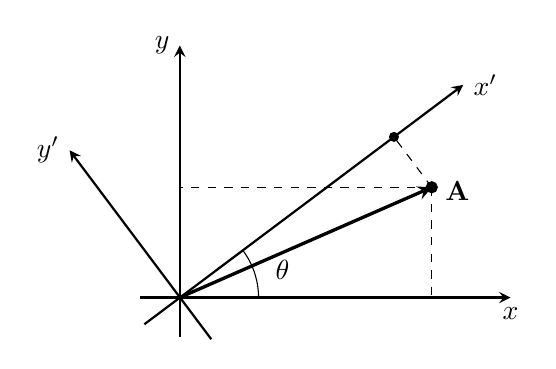
\begin{tikzpicture}[x=1.0cm,y=1.0cm,>=stealth]
  \draw[thick,->] (-0.5,0) -- (4.2,0) node[below] {$x$};
  \draw[thick,->] (0,-0.5) -- (0,3.2) node[left] {$y$};
  \draw[thick,->] (-0.45,-0.34) -- (3.6,2.7) node[right] {$x'$};
  \draw[thick,->] (0.4,-0.53) -- (-1.4,1.87) node[left] {$y'$};
  \draw[very thick,->] (0,0) -- (3.2,1.4);
  \draw[fill] (3.2,1.4) circle (2pt);
  \node[right] at (3.25,1.35) {$\mathbf{A}$};
  \draw[dashed] (3.2,1.4) -- (3.2,0);
  \draw[dashed] (3.2,1.4) -- (0,1.4);
  \draw[dashed] (3.2,1.4) -- (2.72,2.04);
  \draw[fill] (2.72,2.04) circle (1.6pt);
  \draw[thin] (1.0,0) arc[start angle=0,end angle=36.87,radius=1.0];
  \node[right] at (18:1.15) {$\theta$};
\end{tikzpicture}
\end{center}

ছবিতে একই ভেক্টর $\mathbf{A}$ দুটি ব্যবস্থায় দেখা হচ্ছে। পুরনো অক্ষে তার
উপাংশ পাওয়া যায় নিচের ও বাঁয়ের ভাঙা রেখা থেকে; নতুন অক্ষে $x'$ বরাবর
অভিক্ষেপটি দেখানো হয়েছে ছোট বিন্দুটি দিয়ে। তীরটি নড়েনি, কেবল তাকে মাপার
জালিটা ঘুরে গেছে।

\begin{remark}
এখানে ম্যাট্রিক্সকে কেবল একটি সংক্ষিপ্ত লেখার উপায় হিসেবে আনা হলো। তার
নিজস্ব বিস্তৃত তত্ত্ব আছে (গুণের নিয়ম, বিপরীত ম্যাট্রিক্স, eigenvalue), যা
এই সিরিজে নেই। তবু এটুকু জেনে রাখা দরকার, কারণ পদার্থবিজ্ঞানের বইয়ে ঘূর্ণন,
জড়তার ভ্রামক ও পীড়ন সবই ম্যাট্রিক্স আকারে লেখা থাকে, আর ২১ নম্বর
অধ্যায়ে ভেক্টর ক্ষেত্র নিয়ে কাজ করার সময় এই লেখার ভঙ্গিটাই সুবিধা দেবে।
\end{remark}

\begin{example}
$\mathbf{A} = 3\hat{\mathbf{x}} + 4\hat{\mathbf{y}}$ এবং অক্ষ
$\theta = 53.13^{\circ}$ কোণে ঘোরানো হলো (যেখানে $\cos\theta = 0.6$,
$\sin\theta = 0.8$)। নতুন উপাংশ নির্ণয় করো।
\end{example}

\begin{solbox}
\[
  \begin{pmatrix} A_{x}' \\ A_{y}' \end{pmatrix}
  = \begin{pmatrix} 0.6 & 0.8 \\ -0.8 & 0.6 \end{pmatrix}
  \begin{pmatrix} 3 \\ 4 \end{pmatrix}
  = \begin{pmatrix} 1.8+3.2 \\ -2.4+2.4 \end{pmatrix}
  = \begin{pmatrix} 5 \\ 0 \end{pmatrix} .
\]
অর্থাৎ নতুন ব্যবস্থায় ভেক্টরটি পুরোপুরি $x'$-অক্ষ বরাবর, আর তার উপাংশ
$5$। যাচাই: $|\mathbf{A}| = \sqrt{9+16} = 5$, বদলায়নি।

এটিই অক্ষ বেছে নেওয়ার শক্তি: উপযুক্ত ঘূর্ণনে একটি উপাংশ শূন্য করে দেওয়া যায়
এবং সমস্যাটি অর্ধেক হয়ে যায়।
\end{solbox}

\prob{3} $\mathbf{A} = \hat{\mathbf{x}} + \sqrt{3}\,\hat{\mathbf{y}}$।
\begin{enumerate}
  \item অক্ষ $30^{\circ}$ ঘোরালে নতুন উপাংশ নির্ণয় করো।
  \item দৈর্ঘ্য বদলায়নি, যাচাই করো।
  \item নতুন ব্যবস্থায় $\mathbf{A}$ কত কোণ করে $x'$-অক্ষের সঙ্গে?
\end{enumerate}

\begin{sol}
\begin{enumerate}
  \item $\cos 30^{\circ} = \dfrac{\sqrt{3}}{2}$,
        $\sin 30^{\circ} = \dfrac{1}{2}$, তাই
        \[
          A_{x}' = 1 \cdot \frac{\sqrt{3}}{2} + \sqrt{3}\cdot\frac{1}{2}
          = \sqrt{3}, \qquad
          A_{y}' = -1 \cdot \frac{1}{2} + \sqrt{3}\cdot\frac{\sqrt{3}}{2}
          = 1 .
        \]
  \item $\sqrt{3+1} = 2$ এবং মূল দৈর্ঘ্য $\sqrt{1+3} = 2$। সমান।
  \item $\tan\alpha' = \dfrac{1}{\sqrt{3}}$, তাই $\alpha' = 30^{\circ}$।

        মিলিয়ে দেখো: মূল ব্যবস্থায় $\tan\alpha = \sqrt{3}$, অর্থাৎ
        $\alpha = 60^{\circ}$। অক্ষ $30^{\circ}$ ঘোরানোয় কোণটি
        $30^{\circ}$ কমে গেছে, ঠিক যেমন হওয়ার কথা।
\end{enumerate}
\end{sol}

\prob{4} ঘূর্ণন ম্যাট্রিক্স ব্যবহার করে প্রমাণ করো যে
$\mathbf{A}'\cdot\mathbf{B}' = \mathbf{A}\cdot\mathbf{B}$, অর্থাৎ dot product
অক্ষের ঘূর্ণনে বদলায় না। এই ফলটির তাৎপর্য কী?

\begin{sol}
সংক্ষেপে $c = \cos\theta$, $s = \sin\theta$ লিখি। তখন
\[
  A_{x}' = cA_{x}+sA_{y}, \quad A_{y}' = -sA_{x}+cA_{y} ,
\]
এবং $\mathbf{B}$-এর জন্যও একই। গুণ করে যোগ করি:
\[
  A_{x}'B_{x}' = c^{2}A_{x}B_{x} + cs\left( A_{x}B_{y}+A_{y}B_{x} \right)
  + s^{2}A_{y}B_{y} ,
\]
\[
  A_{y}'B_{y}' = s^{2}A_{x}B_{x} - cs\left( A_{x}B_{y}+A_{y}B_{x} \right)
  + c^{2}A_{y}B_{y} .
\]
যোগ করলে আড়াআড়ি পদগুলো কাটাকাটি যায় এবং $c^{2}+s^{2} = 1$ ব্যবহার করে
\[
  A_{x}'B_{x}' + A_{y}'B_{y}' = A_{x}B_{x} + A_{y}B_{y} .
\]

তাৎপর্য: dot product-এর মান কোন অক্ষে হিসাব করা হলো তার উপর নির্ভর করে না,
অর্থাৎ সে একটি সত্যিকারের scalar। এই কারণেই কৃতকাজ, শক্তি বা flux ধরনের
রাশিগুলো সবার কাছে একই আসে, যদিও উপাংশগুলো একেকজনের কাছে একেক রকম।
$\mathbf{B} = \mathbf{A}$ বসালে বিশেষ ক্ষেত্র হিসেবে দৈর্ঘ্যের অপরিবর্তনীয়তাও
পাওয়া যায়, যা প্রথম অনুচ্ছেদে সংখ্যা দিয়ে দেখা গিয়েছিল।
\end{sol}

\end{document}